% section Evaluation

\begin{figure*}[t]
  \subfloat[Heterogeneous functions.   \label{fig:heterogen} ]
  {  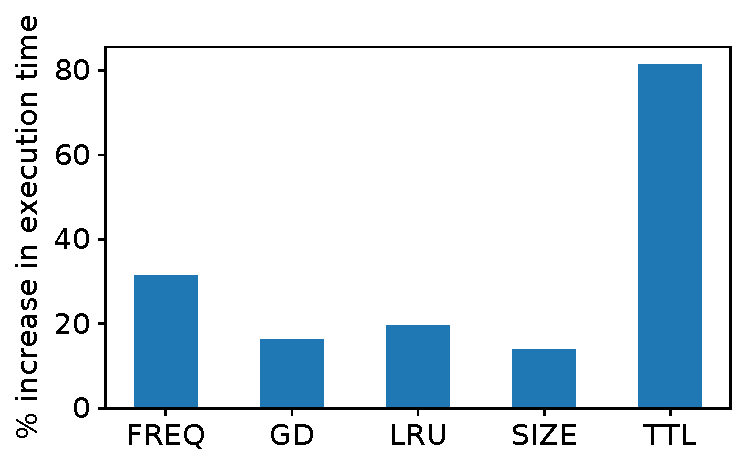
\includegraphics[width=0.25\textwidth]{../graphs/heterogen.pdf} }
  \hfill
  \subfloat[Different initialization times.   \label{fig:diff-warm} ]
  {  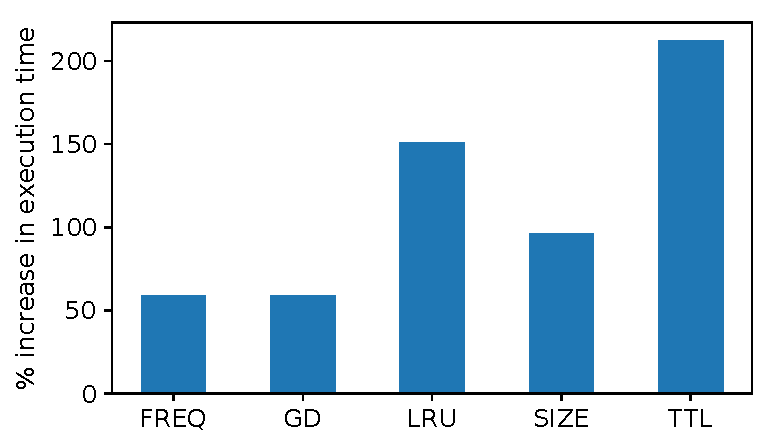
\includegraphics[width=0.25\textwidth]{../graphs/diff-warm.pdf}}
  \hfill
  \subfloat[Our policy provides better performance at higher inter-arrival times.  \label{fig:iat-scaling} ]
  {  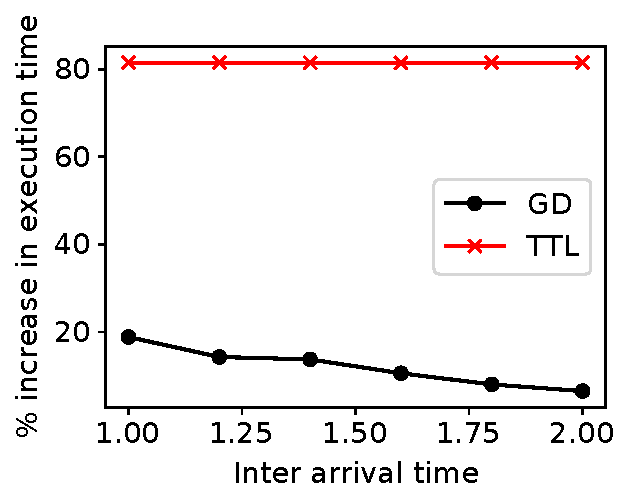
\includegraphics[width=0.22\textwidth]{../graphs/iat-scaling1.pdf}}
  \hfill
  \subfloat[The ``Miss-rate curve'' with our Greedy-Dual policy.
  \label{fig:mrc} ]
  {  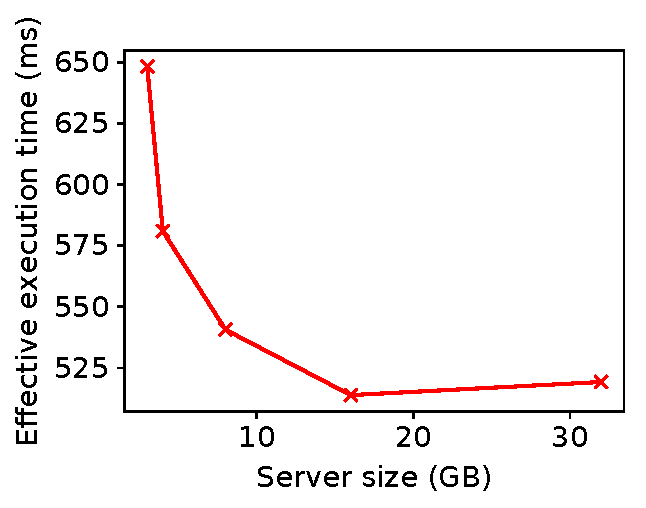
\includegraphics[width=0.22\textwidth]{../graphs/mrc1.pdf}}
  \hfill
    \vspace*{\subsecspace}
  \caption{Keep-alive policy comparison.}
  \label{fig:all}
  \vspace*{\subsecspace}
\end{figure*}


We now present preliminary evaluation of our caching-inspired keep-alive policy. 
%
%We are interested in evaluating its feasibility and effectiveness in serverless environments.
%
We have implemented our Greedy-Dual keep-alive policy described in the previous section, as well as its various variants. 
%
We evaluate all keep-alive policies in a simulation framework that allows us to evaluate their effectiveness for different mixes of functions with different initialization times, memory sizes, invocation frequency, and inter-arrival times. 
%We have also implemented a simulation framework that allows us to evaluate different policies for  various workloads. 
%With our simulator, we can evaluate performance with different function characteristics such as their size, total execution time, initialization time, frequency of invocation, and inter-arrival time.
\emph{We are primarily interested in the increase in the effective execution time of functions due to  cold starts. }
To understand the tradeoffs and differences between various caching-inspired keep-alive policies, we examine different variants of the Greedy-Dual policy:
\vspace*{-5pt}
\begin{description}
  \setlength{\itemsep}{0pt}
\item[GD:] Greedy-Dual policy described in the previous section
\item[FREQ:] Priority=Clock + Frequency. Ignores initialization cost and size. 
  \item [LRU:] Classic least recently used based termination. Ignores size and cost. 
  \item[SIZE:] Considers recency and size, and ignores frequency and cost.
  \item[TTL:] AWS Lambda policy with a fixed ``time to live'' of 30 minutes. 
\end{description}



\noindent \textbf{Heterogeneous functions.}
We first evaluate the effectiveness of keep-alive policies when there is a large heterogeneity in function characteristics.
This is a key characteristic of FaaS platforms, since a single physical server may run 100s of different kinds of functions. 
We use four function classes that are representative of commonly deployed FaaS functions as shown in Table~\ref{tab:workloads}. 
The function  memory sizes range from $[10,1000]$ MB, and running times ranging from $[10, 1000]$ ms. 
Figure~\ref{fig:heterogen} shows this increase in execution time for the various keep-alive policies.
We can see that the function execution time for the various caching-inspired policies is much lower (by up to $4\times$) than the constant-TTL policy being used by current FaaS platforms. 
%The Greedy-Dual policy is able to reduce the increase in execution time due to cold starts by $4\times$ compared to the constant-TTL policy 


Interestingly, for the above  configuration, we see that simpler policies such as SIZE are as effective as the full Greedy-Dual policy. 
The SIZE policy simply terminates the largest containers first---this is extremely effective in our heterogeneous configuration that has very large (1000 MB) containers, which is $100\times$ bigger than the smallest container.  
In cases of such extreme size heterogeneity, terminating a single big container can make room for lots of other smaller containers, and thus SIZE can be a competitive keep-alive policy. 

% In fact, the Greedy-Dual policy performs slightly worse than the simpler SIZE policy (by about 5\%).
% This surprising observation can be explained by considering the following scenario. 
% Suppose the server is full, and a new, large function arrives. The size policy would just terminate the largest container, and thus only one container is terminated. 
% In contrast, because our GD policy terminates containers based on a more nuanced priority, this may result in smaller containers getting terminated before the large containers are terminated to make room for the new function.
% Thus in cases of extreme size heterogeneity, the simpler SIZE policy is also effective.



% \begin{figure}[t]
%   \centering
%   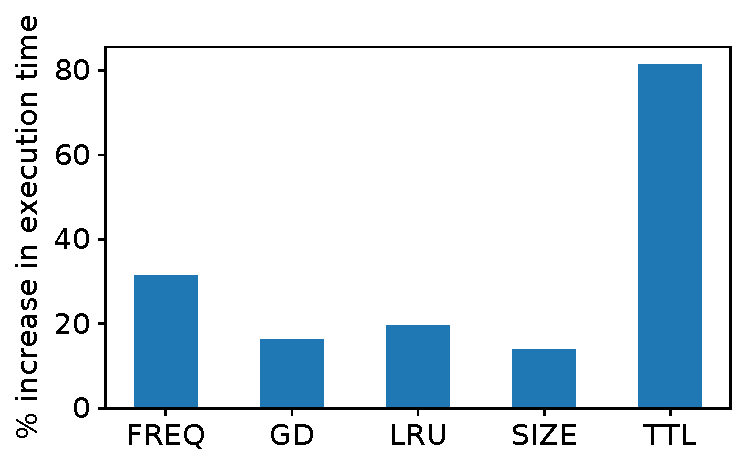
\includegraphics[width=0.35\textwidth]{../graphs/heterogen.pdf}
%     \vspace*{\myfigspace}
%   \caption{Heterogeneous functions}
%   \label{fig:heterogen}
%   \vspace*{\myfigspace}
% \end{figure}


\noindent \textbf{Different Initialization Overheads.} Minimizing the initialization overhead is a crucial task of keep-alive policies.
In this experiment (Figure~\ref{fig:diff-warm}), we consider two function classes that are identical in every way except their initialization overhead (which is in a $1:4$ ratio). 
Because the GD policy considers the initialization overhead when computing the keep-alive priority, it significantly outperforms other policies such as LRU and constant-TTL by $3\times$ and $4\times$ respectively.

We note that based on the workload, simpler policies may match or even outperform our GD policy.
For example, SIZE and LRU in Figure~\ref{fig:heterogen} and FREQ in Figure~\ref{fig:diff-warm}. 
However, the strength of the GD policy is in its generality, and its ability to consistently work well in many different scenarios.



% \begin{figure}[t]
%   \centering
%   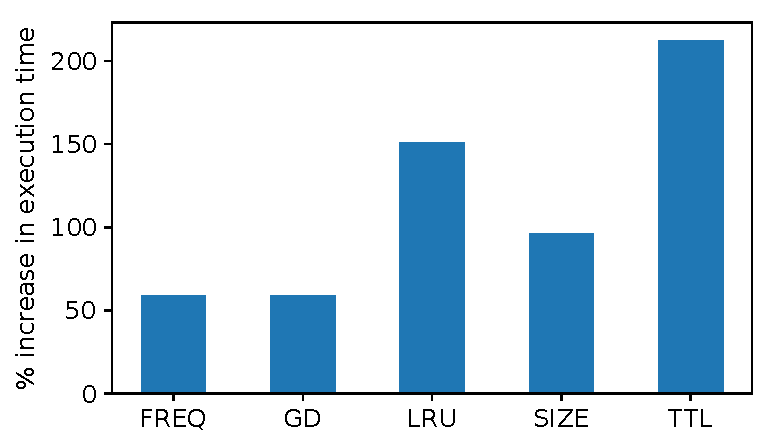
\includegraphics[width=0.35\textwidth]{../graphs/diff-warm.pdf}
%   \vspace*{\myfigspace}
%   \caption{Functions with different initialization times.}
%   \label{fig:diff-warm}
%   \vspace*{\myfigspace}
% \end{figure}


One particular scenario where constant-TTL suffers is when function executions are ``rare'', and their inter-arrival time is longer than the TTL.
In such cases, the containers are terminated, and there is no keep-alive benefit. 
Figure~\ref{fig:iat-scaling} shows the performance of the GD and TTL schemes for different normalized inter-arrival times. 
We can see that as the inter-arrival times increase, the function latencies decrease with GD caching.
However, constant-TTL shows a constant function latency which is more than $8\times$ that of GD.



% \begin{figure}[t]
%   \centering
%   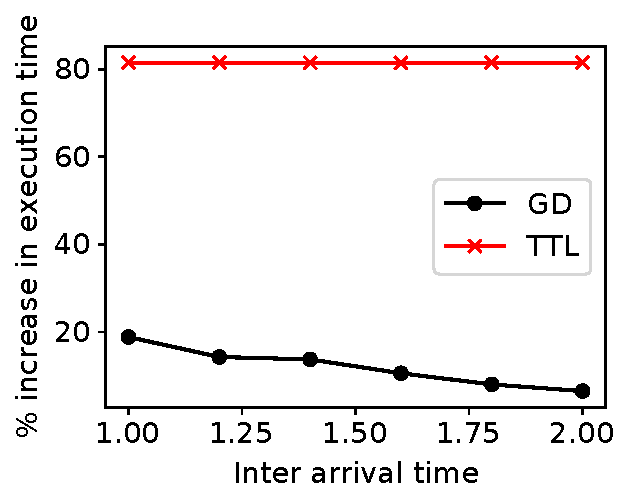
\includegraphics[width=0.33\textwidth]{../graphs/iat-scaling1.pdf}
%   \vspace*{\myfigspace}
%   \caption{As the inter-arrival time of functions increases, our caching effectiveness improves compared to the constant-TTL method.}
%   \label{fig:iat-scaling}
%   \vspace*{\myfigspace}
% \end{figure}



The caching analogy can also be used by FaaS providers for capacity planning.
Figure~\ref{fig:mrc} shows the effective execution time as a function of the server size, which equivalent of a ``miss ratio curve''.
We can see that the server size shows diminishing returns, similar to the classic caching behavior. 

% \begin{figure}[t]
%   \centering
%   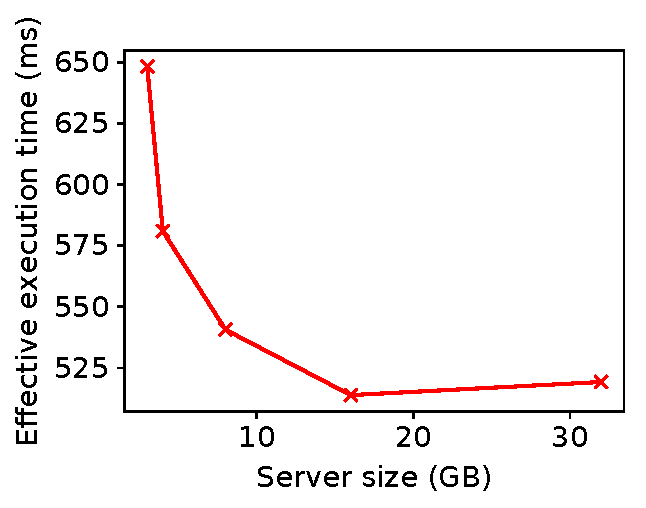
\includegraphics[width=0.33\textwidth]{../graphs/mrc1.pdf}
%   \vspace*{\myfigspace}
%   \caption{The ``Miss-rate curve'' with our Greedy-Dual policy.}
%   \label{fig:mrc}
%   \vspace*{\myfigspace}
% \end{figure}

\vspace*{\subsecspace}
\section{Conclusion}
\vspace*{\subsecspace}

The main insight in this paper is the isomorphism between function keep-alive and object caching.
Using it, sophisticated caching policies can be applied to FaaS.
Our Greedy-Dual based keep-alive policy can reduce cold start overheads by up to $4\times$ compared to simple policies.
The caching analogy can also be used to enhance resource provisioning. 
%As the diversity of FaaS applications and usecases grows, 

%%% Local Variables:
%%% mode: latex
%%% TeX-master: "paper"
%%% End:
